\documentclass[]{../../../../tex/classes/homework}
\usepackage{../../../../tex/packages/hebrewSupport}
\usepackage{../../../../tex/packages/mathShortcuts}

\usetikzlibrary{graphs}
\usepackage{halloweenmath}
\newcommand\ff{\mathrm{f}}
\newcommand\gcc{G^{\mathrm{SCC}}}
\newcommand\squigT{\overset{T}{\squig}}
\newcommand\squigd{\leftrightsquigarrow}
\DeclareMathOperator{\low}{low}

\author{שחר פרץ}
\title{\textit{תרגיל בית 2} $\sim$ אלגוריתמים}
\begin{document}
	\maketitle
	\subsection*{סימונים לבודק}
	\begin{itemize}
		\item לא פתרתי במקור את השאלות לפי הסדר, ובאמצע התרגיל התחלתי להשתמש בנוטציה של $\squigd$ במקום $\squig$ (למסלולים) ו־$-$ במקום $\to$ (לקשתות) בגרפים לא מכוונים. כל שאלה תהיה קונסיסטנטית בסימונים שלה, אבל התרגיל כולו לאו דווקא. 
		\item זמן גילוי בעץ DFS מסומן ב־$\dd[v]$ וזמן סיום עיבוד ב־$\ff[v]$. 
	\end{itemize}
	
	\section{}
	יהיה גרף לא מכוון $G = (V, E)$. נוכיח או נפריך את הטענות הבאות עליו: 
	\begin{enumerate}[(A)]
		\item טענה: אם $G$ קשיר חזק אז בהכרח באף ריצת DFS על $G$ לא תהיינה קשתות חוצות. \begin{proof}[הפרכה]
			נתבונן בגרף הבא: 
			\begin{center}
				\sen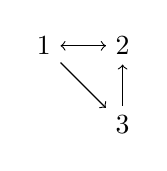
\begin{tikzpicture}
					\graph {1 -> {2, 3}, 3 -> 2, 2 -> 1};
				\end{tikzpicture}\she
			\end{center}
			
			נבחין שריצת DFS אפשרית תתחיל מ־$1$, תעבור ל־$2$, אך שם ''תתקע`` משום שאין קשת ל־$3$ ו־$1$ מסומן באפור. לאחר מכן היא תחזור ל־$1$ ותמשיך לבצע ממנו DFS-visit על $3$ הלבן, דרכו היא תעלה את הקשת $3 \to 2$ שנותרה. נקבל גרף $G_\pi$ כדלהלן: 
			\begin{center}
				\sen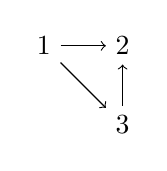
\begin{tikzpicture}
					\graph {1 -> {2, 3}, 3 -> 2};
				\end{tikzpicture}\she
			\end{center}
			נבחין שהקשת $(3, 2)$ היא קשת חוצה: האינטרוואל של $2$ הוא $I_2 = [2, 2]$ בעוד האינטרוואל של $3$ הוא $I_3 = [4, 4]$ (ו־$I_1 = [1, 5]$). אלו שני אינטרוואליים שהחיתוך בינהם ריק ולכן הקשת בינהם חוצה. 
		\end{proof}
		\item טענה: אם בכל ריצת DFS על $G$ מתקיים $\ff[u] > \ff[v]$ אז בהכרח יש מסלול מכוון מ־$u$ ל־$v$ ב־$G$. \begin{proof}
			נוכיח את הקונטראפוסיטיב. יהיו $u, v$ בינהם לא קיים מסלול מכוון. נבחר את סדר הריצה של ה־DFS כך שנתחיל את ה־DFS-visit הראשון מ־$u$. נבחין שאותה הריצה של ה־DFS-visit תחזור ללולאה המקורית בזמן $\ff[u] = t$ לפני גילוי $v$, שכן אחרת גילינו דרך $u$ את $v$, ומכאן ש־$I_v \subset I_u$, ומעקרון המסלול הלבן יש מסלול לבן בינהם, אך הנחנו שאין אף מסלול בין שניהם. מכאן ש־$\ff[v]$ יתרחש רק לאחר זמן $t$, כלומר $\ff[v] \ge \ff[u]$, וסיימנו. 
		\end{proof}
	\end{enumerate}
	
	\npage
	
	\section{}
	נתון גרף $G = (V, E)$ וצומת $s \in V$, כך שכל הצמתים ב־$V$ נגישים דרך $s$. נוכיח או נפריך את הטענות הבאות. 
	\begin{enumerate}[(A)]
		\item טענה: אם $G$ לא מכוון, וקיימים עץ BFS ועץ DFS מ־$s$ זהים $T$, אז $G = T$.
		\begin{proof}[הפרכה למקרה בו הגרף אינו פשוט]
			במקרה והגרף אינו פשוט, הגרף $G = (V, E)$ כך ש־$V = \{1, 2\}$ ו־$E = \{\{1, 2\}, \{1, 2\}\}$ יקיים את הנדרש (כאשר למרבה הפלא $G_{\pi}  = (V, E')$ מקיים ש־$E = \{\{1, 2\}\}$ בעבור כל $s$). 
		\end{proof}
		במקרה שבו הגרף אינו פשוט (אני מניח שזו הייתה הכוונה בשאלה, אבל אם לא, תתעלמו מהפסקה למטה), נוכל להוכיח את הטענה:
		 \begin{proof}[הוכחה בהנחה שהגרף פשוט]
			נראה ש־$G$ עץ, ומכאן ההוכחה תהיה פשוטה. קל לראות ש־$G$ גרף קשיר שכן DFS מבקר בכל הקודקודים בגרף, בעוד BFS יבקר בכל הקודקודים בגרף (הלא מכוון) אמ''מ הוא גרף קשיר (מנכונות אלגוריתם למציאת רכיבי קשירות), ומכאן שעצי ה־DFS וה־BFS יהיו זהים אמ''מ $G$ קשיר. 
			
			עתה נוכיח ש־$G$ חסר מעגלים. נניח בשלילה שב־$G$ יש מעגל באורך $n$. נניח שבזמן $t$ מתגלה הצומת הראשון במעגל $v_1$ (כלומר $\dd[v] = t$). בעת כלשהי בעת הרצת DFS-visit על $v$ (כלומר לפני $\ff[v]$), בהכרח נמצא $v_2$ כלשהו נוסף על המעגל, כי בינו לבין $v$ יש מסלול לבן בזמן $\dd[v]$. באינדוקציה, נבחין שבין $v_i$ לבין יתר צמתי המעגל שלא נמצאו יש מסלול לבן ב־$\dd[v_i]$, ולכן קיים $v_{i + 1}$ על המעגל שימצא לאחר $v_i$. סה''כ, נוכל למצוא קודקודים $v_1 \dots v_n$ כך ש־$I_{v_1} \subset I_{v_2} \subset \cdots \subset I_{v_n}$. כלומר, ישנו מסלול (מכוון ב־$G_{\pi}$, כי זהו תמיד גרף מכוון) $v_1 \to v_2 \squig v_n$, ומהשוויון, גם בגרף ה־BFS. מכאן שיש מק''ב $s \squig v_1 \squig v_n$, באורך $\dg(s, v_1) + n$, אך המסלול $s \squig v_1 \to v_n$ (שקיים כי $v_1 \dots v_n$ מעגל) קצר יותר (בהנחה ש־$n > 2$, שכן אחרת ישנן קשתות חוזרות והגרף איננו פשוט). 
		\end{proof}
		\item טענה: אם $G$ DAG, וקיימים עץ BFS ועץ DFS מ־$s$ זהים $T$, אזי בהכרח $G =T$.
		\begin{proof}[הפרכה, גם במקרה הלא פשוט]
			נתבונן בגרף הבא (פעם שנייה שהוא מופיע בתרגיל הזה. גרף מועיל): 
			\begin{center}
				\sen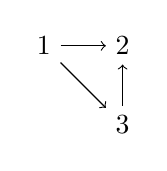
\begin{tikzpicture}
					\graph {1 -> {2, 3}, 3 -> 2};
				\end{tikzpicture}\she
			\end{center}
			הרצת DFS אפשרית על הגרף תתחיל מ־$s = 1$, תבקר ב־$2$, תתקע, תחזור ל־$1$ כדי להמשיך ממנו ל־$3$, להתקע, לחזור ל־$1$, להתקע גם שם ולסיים את הריצה. הרצה כזו תותיר אותנו עם הגרף $G_{\pi} = (V, E')$ כאשר $E' = \{\{1, 2\}, \{1, 3\}\}$. קל לראות שזהו גרף הרצת BFS מ־$s=1$, שכן המק''ב היחיד מ־$1$ ל־$2$ הוא $1 \to 2$ והמק''ב היחיד מ־$1$ ל־$3$ הוא $1 \to 3$. עם זאת, $G \neq G_\pi$ שכן $\{2, 3\} \notin E'$. זאת למרות שכל הצמתים בגרף נגישים מ־$s$ באמצעות מסלול כלשהו, ושאין אף מעגל (במובן המכוון) בגרף. 
		\end{proof}
		\item אם $G$ מכוון וחסר מעגלים, ומתקיים $\sof E > \sof V - 1$, אזי בהכחר קיימים עץ BFS ועץ DFS מ־$s$, נסמנם $T_1, T_2$, כך ש־$T_1 \neq T_2$. 
		\begin{proof}
			נריץ BFS \textit{כלשהו} על $G$ מ־$s$ לקבלת עץ BFS $T_1 =: G_\pi$. משום ש־$\sof E > \sof V - 1$, ו־$G_\pi$ עץ, קיימת $(u, v) := e \in E$ שאינה ב־$G_\pi$. משום שהרצנו BFS דרך $s$ קיים מסלול פשוט (למעשה, קצר ביותר) $s \squig u$ שעובר דרך קשתות $G_\pi$ בלבד, ובפרט לא דרך $e$. אך יתרה מכך, ניתן להוכיח שהוא אינו עובר ב־$v$: אם הוא עובר ב־$u$ אז מצאנו מסלול $s \squig v \squig u$ שלא עובר ב־$u \to v$, ולכן $v \squig u \to v$ מעגל פשוט, וזו סתירה לכך ש־$G$ חסר מעגלים. 
			
			עתה אנו מחזיקים במסלול פשוט, שלא חוזר על אף קודקוד פעמיים, והוא $s \squig u \to v$. נשתמש בו כדי לקבוע את הסדר בלולאה הפנימית של ה־DFS (ולאחריו, בסדר כלשהו), ונריץ DFS מ־$s$ (שאר סדר הלולאה החיצונית שלא משנה). נבחין שמשום שהוא לא חוזר על אף קודקוד פעמיים, תמיד ה־DFS יתקל בצומת לבנה וימשיך לעבוד לפי סדר המסלול. בפרט, ה־DFS יוסיף לעץ שלו $T_2$ את $u \to v$, על אף שקשת זו לא שייכת ל־$T_1$. 
			
			סה''כ מצאנו $T_1, T_2$ מתאימים, שניהם יוצאים מ־$s$, ומתקיים בעבורם $T_1 \neq T_2$. 
		\end{proof}
	\end{enumerate}
	
	\npage
	\section{}
	מסלול המילטון הוא מסלול פשוט העובר פעם אחת בדיוק בכל צומת בגרף. יהי $G$ DAG. 
	\begin{enumerate}[(A)]
		\item נוכיח שאם קיים מסלול המילטון בגרף אז יש סדר מיון טופולוגי יחיד. \begin{proof}
			\begin{itemize}
				\item \textbf{קיום: }נמיין טופולוגית לפי מסלול ההמילטון. משום שזהו מסלול $v_1 \dots v_n$, בהכרח כל מסלול $v_1 \squig v_n$ יופיע לפי הסדר, ואם בשלילה קיים מסלול הפוך בכיוון המסלול $v_j \squig v_{i}$ בעבור $i < j$, אז מהיות מסלול ההמילטון מסלול, הוא מכיל מסלול $v_j \squig v_i$, וסה''כ מצאנו מעגל $v_j \squig v_i \squig v_j$ וזו סתירה להיות הגרף DAG. 
				\item \textbf{יחידות: }נתבונן במיון הטופולוגי $v_1 \dots v_n$ לעיל. נתבונן ב־$v_{i + 1}$. נוכיח באינדוקציה שהוא חייב לבוא אחרי $v_i$, שכן אם בשלילה קיים בינהם $v_j \neq v_{i + 1}$ במיון טופולוגי אחר (מה.א. מתקיים $v_{j > i}$, שכן הצמתים לפני $i$ מקובעים), ש־$v_i$ מופיע לפניו ו־$v_{i + 1}$ אחריו. ידוע שמסלול ההמילטון עובר $v_1 \to v_2 \squig v_i \to v_{i +1} \squig v_j$. לכן מצאנו מעגל $v_j \to v_{i + 1} \squig v_j$, אך אנו ב־DAG, ולכן לא קיים $v_j$ כזה. 
				
				בסיס האינדוקציה נובע ישירות מהצעד: אם $v_{i + 1}$ חייב לעקוב אחר $v_i$, אז בפרט $v_2$ מופיע מיד לאחר $v_1$. 
				
				משום שיש מספר סופי של קודקודים, המיון היחיד שייתכן במצב שבו $v_{i + 1}$ תמיד עוקב את $v_i$ במיון הטופולוגי, הוא המיון שמצאנו ממסלול ההמילטון. 
			\end{itemize}
		\end{proof}
		\item נוכיח שאם סדר המיון הטופולוגי יחיד, אז הוא מהווה מסלול המילטון. \begin{proof}
			די להראות שהסמ''ט הינו מסלול, שכן הסמ''ט כולל את כל הצמתים בגרף. יהי סמ''ט $v_1 \dots v_n$ ונניח שהוא יחיד. נניח בשלילה שלא קיימת קשת $v_i \to v_{i + 1}$. אז נבחין ש־$v_1 \dots v_{i + 1}, v_i, \dots v_n$ סמ''ט שנסמנו $w_1 \dots w_n$; לכל מסלול $v_k \squig v_m$ מתקיים $k<m$ במסלול המקורי, ומכאן שכל מסלול $w_k \squig w_m$ מקיים $k < m$ שכן אם המסלול יכול לכלול רק אחד מבין $w_i$ או $w_{i + 1}$. 
		\end{proof}
		\item נתאר אלגוריתם יעיל ככל הניתן למציאת מסלול המילטון בגרף. 
		\begin{itemize}
			\item \textbf{אלגוריתם: }ראינו בהרצאה אלגוריתם למציאת סמ''ט בגרף. נריץ אותו, ונחזיר את הקודקודים לפי סדר הסמ''ט להיות מסלול ההמילטון בגרף, במידה והם אכן משרים מסלול (כלומר נבדוק האם ישנה קשת $v_i \to v_{i + 1}$). 
			\item \textbf{סיבוכיות: }האלגוריתם מההרצאה מתבסס על הרצת DFS ורץ בסיבוכיות $\oc(\sof V + \sof E)$. המעבר על צמתי הסמ''ט והחזרתם תיארך $\sof V$ פעולות בזמן קבוע. סה''כ האלגוריתם ירוץ בסיבוכיות של $\oc(\sof V + \sof E)$. 
			\item \textbf{נכונות: }הוכחנו בסעיפים קודמים שקיים מסלול המילטון בגרף אמ''מ הסמ''ט יחיד והוא מסלול ההמילטון. מכאן שכאשר יש מסלול המילטון בגרף, האלגוריתם בהכרח ימצא אותו להיות צמתי הסמ''ט לפי סדרם, ובמידה ואין מסלול המילטון בגרף, האלגוריתם יזהה שצמתי הסמ''ט לפי סדרם לא משרים מסלול ויחזיר תשובה שלילית. יש לציין שתמיד נמצא סמ''ט לבצע את הבדיקה הזו עליו, כי $G$ הוא DAG. 
		\end{itemize}
	\end{enumerate}
	
	\npage
	\section{}
	נתון גרף לא מכוון $G = (V, E)$ שהרצת DFS עליו פלטה גרף $G_{\pi}$. נגדיר \textit{אב חורג} של $v$ (ביחס להרצת ה־DFS) להיות צומת אליה מ־$v$ יש קשת אחורית ל־$w$. 
	\begin{enumerate}[(A)]
		\item יהי מסלול פשוט $u_0 - u_1 - \cdots - u_k$ ביער $G_\pi$. נסמן $G' = (V, E \setminus \{u_{k - 1}, u_k\})$. 
		
		טענה: $u_0$ ו־$u_k$ באותו רכיב הקישורת אמ''מ ל־$u_k$ יש צאצא ב־$G_\pi$ עם אב חורג $w \in V$ המקיים $\dd[w] \le \dd[u_{k - 1}]$. 
%		טענה: $u_0$ ו־$u_k$ באותו רכיב הקשירות אמ''מ קיים $i \in 0 \dots {k - 1}$ כך ש־$u_i$ אב חורג של בן $v$ כלשהו של $u_k$, המקיים $\dd[v] \ge \dd[u_k]$. 
		\begin{proof}
			נוכיח את שני הכיוונים. 
			\begin{itemize}
				\item[$\implies$]אם קיים ל־$u_k$ יש צאצא $v$ עם אב חורג $w$ המקיים $\dd[w] \le \dd[u_{k - 1}]$, אזי יש מסלול $u_k \squigd v $ (שבהכרח לא כולל את הקשת $\{u_{k - 1}, u_k\}$, שכן הוא מסלול מצומת לצאצא בעץ, ולכן אין סיבה ש''יטפס`` מעלה לצומת שהסרנו) וקשת אחורית $v - w$. בהכרח ב־$G$ ישנו מסלול כלשהו $w \squigd u_0$, שכן המסלול $u_0 \squigd u_k \squigd v - w$ מסלול ב־$G$ (אך לא ב־$G'$) ואנו בגרף לא מכוון. לכן שניהם נמצאים באותו עץ ה־DFS. נשאף למצוא מסלול שלא עובר ב־$u_{k - 1} - u_k$; בגלל ש־$\dd[u_0] \le \dd[w] \le \dd[u_{k - 1}]$ (כי $u_0$ השורש), ומעקרון המסלול הלבן פעמיים, קיים מסלול $u_0 \squigd w$ כך שבעת ההגעה ל־$w$ מ־$u_0$, עדיין $u_{k - 1}$ לבן, כלומר לא הגענו אליו וגילינו את הקשת $u_{k - 1} - u_k$. לכן סה''כ שרשור המסלולים: 
				\[ u_k \squigd v \squigd w - u_{k - 1} \squigd u_0 \]
				הוא מסלול ללא הקשת $u_{k - 1} - u_k$ ולכן מופיע ב־$G$. 
%				אם קיים $i \in [n - 1]$ כך ש־$u_i$ אב חורג של $u_k$, אז ישנו מסלול פשוט $u_0 \squig u_i$ (זה נתון), וכן קשת (אחורית, ובפרט קשת בגרף המקורי) $\{u_i, u_k\}$ וסה''כ ישנו מסלול $u_0 \squig u_i \to u_k$ וסיימנו. 
				\item[$\impliedby$]נניח $u_0, u_k$ באותו רכיב קשירות ב־$G'$. נסמן ב־$G_\pi'$ את $G_\pi$ ללא הקשת $\{u_{k - 1}, u_k\}$. 
				
				נניח שלא קיים אף צאצא ב־$G_\pi$ המקיים את הנדרש לעיל. בעת הסדרת $u_{k -1} - u_k$ מ־$G$, בגלל ש־$G_{\pi}$ יער, ניצור שני רכיבי קשירות נוספים ב־$G_\pi'$: האחד, $T_0$ שיקיים $u_{k - 1} \in T_0$ (ומשום ש־$u_0 \squigd u_{k -1}$ מסלול ב־$G'$ וב־$G_\pi$, ובפרט ב־$G_\pi'$, גם $u_0 \in T_0$) והשני, $T_k$ שיקיים $u_k \in T_k$. נוכיח שאין קשתות שיוצאות מ־$T_k$ ל־$T_0$ ב־$G$ כולו (מובן שאין בתת־הגרף $G_\pi'$, שכן אלו רכיבי קשירות שונים שלו). תהי $(v, w) = e \in E'$ כך ש־$v \in T_0$ (קשת היוצאת מ־$T_0$): 
				\begin{itemize}
					\item אם $w \in T_k$, סיימנו. 
					\item אם $w \notin T_k$ וגם $w \notin T_0$, אז $w$ ברכיב קשירות של $G_\pi$ המקורי השונה מזה ש־$u_0$ בו, ומשום שאנו בגרף לא מכוון, אין מסלול מרכיב קשירות זה בכל $G$ חזרה ל־$T_0$, וסיימנו. 
					\item אחרת $w \in T_0$. בגלל המשפט לקטעים מקוננים, מתקיים ש־$\dd[w] > \ff[u_k] \ge \dd[u_k]$ (זאת כי מהנחת השלילה $\dd[w] \ge \dd[u_k]$, וכי $w$ לא בן של $u_k$). בגלל ש־$v \in T_k$ הוא צאצא של $u_k$ ב־$G_\pi'$ (כי $u_k$ השורש של $T_k$) ואז $\ff[u_k] > \ff[v] \ge \dd[v] > \dd[u_k]$. נשלב את אי־השוויונות ונקבל $\dd[w] > \dd[v]$. מכאן ש־$e$ קשת עץ כלומר $T_0$ ו־$T_k$ מחוברים ב־$G_\pi'$, וזו סתירה לכך שאלו רכיבי קשירות שונים. 
					
					סה''כ $T_0$ לא נגיש מתוך $T_k$ ב־$G'$ כולו. בפרט $u_k \in T_k$ לא נגיש ע''י $u_0 \in T_0$, ולכן הם נמצאים ברכיבי קשירות שונים ב־$G'$, וזו סתירה להנחה. 
				\end{itemize}
			\end{itemize}
		\end{proof}
		\item נמצא אלגוריתם יעיל למציאת הגשרים בגרף קשיר נתון. 
		\begin{itemize}
			\item \textbf{אלגוריתם: }נריץ את האלגוריתם מהתרגול למציאת ערכי $\low$ בגרף. לכל $\{v, u\} := e \in E$ (נעבור עליהן אחת־אחת), אם מתקיים $ \dd[v] < \low[u]$ במובן הרחב אז נשמור את הקשת כגשר. 
			\begin{itemize}
				\item \textbf{האלגוריתם פולט גשרים בלבד: }נתבונן ב־$\{u, v\} = e$ הנפלטה ע''י האלגוריתם. נתבונן במסלול כלשהו מהשורש ל־$v$, הוא $u_0 \squigd u_{k -2} - v- u$
				\begin{itemize}[*]
					\item אם $\low[u] = \infty$: אז מהסעיף הקודם, לאחר הסרת $v - u$ מהגרף, אין מסלול בין $u$ ל־$u_0$ (אחרת יש צאצא ל־$u$ עם אב חורג, ואז $\dd[u] \neq \infty$) כלומר פיצלנו את הגרף לשני רכיבי קשירות. 
					\item אם $\dd[v] < \low[u]$: אב החורג המינימלי של צאצאי $u$ (נסמנו $w$) יקיים $\dd[v] < \dd[w] = \low[u]$. לכן לא קיים אף אב חורג $w_0$ כך ש־$\dd[w_0] \le \dd[v]$ (זו תהיה סתירה למינימליות של $w$), כלומר ניתן להפעיל את המשפט הקודם ולקבוע מטיעונים דומים שהסרת $v - u$ תגרום לפיצול לשני רכיבי קשירות. 
				\end{itemize}
				\item \textbf{אלגוריתם פולט את כל הגשרים: }תהי $\{u, v\} = e$ ונניח שהיא גשר. אזי נתבונן במסלול $u_0 \squigd u_{k- 2} - v - u$ כאשר $u_0$ השורש. ידוע שניתוק $v - u$ תגרום לכך ש־$u$ ו־$u_0$ יהיו בשני רכיבות שונים (כי $u - v$ גשר). מהמשפט הקודם, ייתכנו שני מקרים: 
				\begin{itemize}[*]
					\item או של־$u$ אין צאצא עם אף אב חורג. במקרה זה מהגדרה $\low[u] = \infty$ והאלגוריתם יחזיר את $u$. 
					\item או של־$u$ יש אב חורג $w$, אך $\dd[v] < \dd[w]$. בגלל ש־$\dd[w] \le \low[u]$ מההגדרה, אז $\dd[v] < \low[u]$ וסיימנו. 
				\end{itemize}
			\end{itemize}
			\item \textbf{סיבוכיות: }הפעלת האלגוריתם למציאת ערכי $\low$ יארך $\oc(\sof V + \sof E)$ בהתאם לתוצאה מהכיתה. מעבר על $E$ ובדיקת אי־שיוונות בזמן קבוע תארך $\oc(\sof E)$. סה''כ $\oc(\sof V + \sof E)$. 
		\end{itemize}
		\item נמצא אלגוריתם יעיל שמוצא את כל הקשתות שמשתתפות במעגל פשוט. 
		\begin{itemize}
			\item \textbf{אלגוריתם: }נריץ את האלגוריתם למעלה למציאת גשרים. אם הקשת אינה גשר, נחזיר אותה. 
			\item \textbf{נכונות: }
			\begin{itemize}
				\item \textbf{כל הגשרים אינם על מעגל פשוט: }בהינתן גשר $\{v, u\}$, אם בשלילה הוא על מעגל פשוט $v - u \squigd v$ אז הסרת $(v, u)$ לא תשמיד את $u \squigd v$ (שכן המעגל פשוט), ומכאן שכל המסלולים שדרשו את הקשת $(v, u)$ יוכלו לעבור ב־$u \squigd v$ באין מפריע. 
				\item \textbf{כל הקשתות על שאינן מופיעות במעגל פשוט הן גשרים: }תהי קשת $e = \{v, u\}$ שאינה מופיעה במעגל פשוט. אם בשלילה היא איננה גשר, אז גם לאחר הסרתה קיים מסלול $v \squigd u$ (אחרת היא מגדילה את מספר רכיבי הקשירות בגרף). אך עתה מצאנו מעגל פשוט $v \squigd u - v$ (כי $u - v$ לא יכולה להשתתף ב־$v \squigd u$ שנקבע לאחר הסרתה), כלומר $\{u, v\}$ על מעגל פשוט וזו סתירה. 
			\end{itemize}
			\item \textbf{סיבוכיות: }עלות הרצת האלגוריתם מהסעיף הקודם היא $\oc(\sof V + \sof E)$. בהינתן פלט $\tl E$ מהסעיף הקודם, חישוב $E \setminus \tl E$ יארך $\sof {\tl E} = \oc(\sof E)$. סה''כ $\oc(\sof V + \sof E)$. 
		\end{itemize}
	\end{enumerate}
	
	\npage
	\section{}
	נתון גרף לא מכוון וקשיר $G = (V, E)$. נניח ש־$G$ חסר גשרים. נוכיח קיום תת־גרף $H =(V, E')$ קשיר וחסר גשרים, כך ש־$\sof{E'} \le 2\sof V - 2$. 
	\begin{proof}
		ניעזר באלגוריתם המוצא את $H$ כדי להוכיח את הטענה. 
		\begin{itemize}
			\item \textbf{אלגוריתם: }נריץ DFS על $G$ לחישוב ערכי $\low$ בהתאם לאלגוריתם מהתרגול ונקבל $G_\pi$. לכל $v \in V$, נוכל להתבונן באב החורג $u$ של הבן ש־$v$ המקיים $\dd[u] = \low[v]$, נסמנו $u_v$. אם $\{v, u_v\}$ קשת ב־$G$, נוסיף אותה ל־$H$. נוסף על כך נוסיף את קשתות העץ של $G_\pi$ ל־$H$. 
			\item \textbf{נכונות: }בבירור $H$ קשיר שכן קשתות $G_\pi$ נמצאות ב־$H$, ו־$G_\pi$ קשיר (כי $G$ קשיר). קל לראות שהוא תת־גרף כי במידה וקשתות הן לא קשתות עץ (שנמצאות ב־$G$) או קשתות מהצורה $\{v, u_v\}$ (שאנו מוסיפים אותה רק אם הן נמצאות ב־$G$), הן לא יכללו ב־$H$. נפנה להוכיח את שתי הטענות העיקריות על הגרף שקיבלנו: 
			\begin{itemize}
				\item \textbf{$\bm{H}$ חסר גשרים: }תהא $\{u, v\} := e \in E'$. ידוע ש־$e$ לא גשר ב־$G$ (כי הוא חסר גשרים), ומשאלה 4 בהכרח $\dd[u_v] = \low[v] \le \dd[u]$ (ובפרט $\low[v]$ סופי). מהגדרת $\low$ קיים לנו צאצא $w$ של $v$ ב־$G_\pi$ (ובפרט ב־$H$) כך ש־$v \squigd w$ וגם יש קשת אחורית מ־$w$ ל־$u_v$ (מכיוון ש־$\low[w] = \dd[u_v]$ וגם $\{w, u_v\}$ בגרף, אז $\{w, u_v\}$ הקשת האחורית ב־$H$). בגלל ש־$u_v$ התגלה לפני $u$ (כי $\dd[u_v] = \low[w] = \low[v] \le \dd[u]$) ושניהם באותו העץ, יש לנו מסלול $u \squigd u_v$ שלא נוגע בצמתים שהתגלו בזמן נמוך מ־$\dd[u]$ (ובפרט זר למסלול $v \squigd w$ שמצאנו מקודם, מ־$v$ לצאצא שלו). סה''כ יש לנו את המעגל הפשוט: 
				\[ v \squigd w - u_v \squigd u - v \]
				ומשום ש־$\{u, v\}$ על מעגל פשוט, היא איננה גשר (גם כן משאלה 4). 
				\item \textbf{מתקיים $\bm{\sof {E'} \le 2 \sof V - 2}$: }נספור את כמות ההוספות שלנו ל־$H$: 
				\begin{itemize}
					\item ראשית, לכל $v$, נוסיף לכל היותר קשת נוספת (אם ישנה קשת אחורית לאב הקדמון המינימלי של הצאצאים שלה, נוסיף קשת אחורית זו). בהכרח לא נוסיף צומת כזו לשורש, כי אם ערך ה־$\low$ שלו קטן מערך הגילוי שלו, אז יש קשת שהתגלתה בזמן גילוי שלילי, וזה לא ייתכן. סה''כ נוסיף לכל היותר $\sof V - 1$ קשתות בשלב זה. 
					\item שנית, את כל $G_\pi$. זהו עץ (פורש) של $G$ ולכן יש בו $\sof V - 1$ קשתות בדיוק. 
				\end{itemize}
				סה''כ הוספנו לכל היותר $\sof V - 1 + \sof V - 1 = 2\sof V - 2$ קשתות ל־$H$, כנדרש. 
			\end{itemize}
		\end{itemize}\envendproof
	\end{proof}
	
	\npage
	\section{}
	יהי גרף לא מכוון $G = (V, E)$ ומספר $k \in \N$. נמצא אלגוריתם יעיל המוצא ת''ק $U \subset V$ כך ש־$\sof U = k$ בעבורה (א) לכל $v \in \ol U$ קיים $u \in U$ כך שיש מסלול מכוון $v \squig u$ ו־(ב) לא קיים מסלול מכוון בין שני צמתים שונים של $U$. 
	\begin{itemize}
		\item \textbf{אלגוריתם: }נחשב את $G^{T}$ ונחפש בו קבוצת מוצא מינימלית $U$ באמצעות האלגוריתם מהתרגול. אם גודל הקבוצה הוא $k$, נחזיר אותה. אחרת, נחזיר אי־קיום. 
		\item \textbf{נכונות: }ראשית נסמן ב־$\squigT$ מסלול ב־$G^{T}$. 
		\begin{itemize}
			\item \textbf{אם האלגוריתם פולט פלט, הפלט תקין: }ראשית, נראה שהפלט הוא אכן קבוצה מגודל $k$ שמקיימת את (א) ו(ב). 
			\begin{enumerate}[(A)]
				\item יהי $v \in \ol U$. נוכיח קיום $u \in U$ כך שישנו מסלול $v\squig u$. ידוע ש־$U$ קבוצת מוצא מינימלית ב־$G^{T}$, כלומר כל קודקוד ובפרט $v$ נגיש מתוכה באמצעות $u \squigT v$ עבור $u \in U$ כלשהו. לאחר מעבר מ־$G^{T}$ ל־$G$, המסלול $u \squigT v$ יהפוך למסלול $v \squig u$, וסיימנו. 
				\item נניח בשלילה שישנו מסלול מכוון $u_1 \squig u_2$ בעבור $u_1, u_2 \in U$ שונים. האלגוריתם למציאת קבוצת מוצא מינימלית מחפש ''מקורות`` שב־$G^{T}$ כל הקשתות מהם יוצאות, כלומר $\din(u) = 0 \land \dout(u) > 0$ ב־$G^{T}$. מכאן שב־$G$ מתקיים $\dout(u) = 0$ עבור $u \in U$ ובפרט עבור $u_1, u_2$. אך המסלול $u_1 \squig u_2$ מסתיים בקשת $? \to u_2$, כלומר $\din(u_2) > 0$ וזו סתירה. 
			\end{enumerate}
			ומאופן פעולת האלגוריתם, ישירות $\sof U = k$. לכן כל פלט של האלגוריתם, תקין. 
			\item \textbf{אם האלגוריתם לא פולט תשובה שלילית, לא קיימת קבוצה מתאימה: }נראה שאם קיימת ת''ק מגודל $k$ מהמקיימת את (א) ו(ב), אזי האלגוריתם יפלוט אותה. נראה ש־$U$ קבוצת מוצא מינימלית ב־$G^{T}$. 
			\begin{itemize}[*]
				\item \textbf{קבוצת מוצא: }לכל $v \in G$, נראה ש־$v$ נגיש מ־$U$. אם $v \in U$ אז $v$ נגיש מעצמו וסיימנו. אם $v \in \ol U$, מ(א) קיים ב־$G$ מסלול $v \squig u$ עבור $u \in U$ כלשהו. לכן ישנו מסלול $u \squigT v$ ו־$v$ נגיש מ־$u$ כנדרש. 
				\item \textbf{מינימלית: }נניח בשלילה שקיימת קבוצת מוצא $U' \subsetneq U$ ב־$G^{T}$ (אפשר לנסח כך דברים כי הראנו ש־$U$ קבוצת מוצא). אזי קיים $v \in U \setminus U'$. ידוע מ(ב) שלא קיימת מסלול מכוון בין $v$ שאר $U'$ ב־$G$, שכן $v \in U$, ומכאן שב־$G^{T}$ לא קיים מסלול היוצא מ־$U'$ ומגיע ל־$v$. כלומר, $v$ לא נגיש מ־$U'$, וזו סתירה. 
			\end{itemize}
		\end{itemize}
		\textbf{שאלה לבודק: }יש דרך יותר טובה לנסח לעיל את הכותרות ''אם האלגו' לא פולט [...]'' ו''אם האלגו פולט פלט הפלט תקין``? (כלומר, האם יש שמות במדמ''ח ל''גרירה דו־כיוונית`` מהסוג הזה). 
		\item \textbf{סיבוכיות: }חישוב $G^{T}$ יארך $\oc(\sof E)$ (אין צורך להעתיק את $V$ שוב). מציאת הקבוצה הפורשת המינימלית המינימלית באמצעות האלגוריתם מהתרגול תיארך $\oc(\sof V + \sof E)$. מניית האיברים בקבוצה הפורשת המינימלית תיארך $\oc(\min\{k, \sof V\})$ (כי נוכל לעצור את הספירה במידה ונעבור את $k$). סה''כ, סיבוכיות האלגוריתם היא $\oc(\sof V + \sof E)$. 
	\end{itemize}
	
	\npage
	\section{}
	יהי וקטור $X = (X_1 \dots X_n)$ של מספרים שלמים חיובים. נגדיר את הפיזור $X$ להיות $\sof{\{X_i \mid 1 \le i \le n\}}$. נתון $m$ א''שים מהצורה $X_j \le X_i$. נמצא אלגוריתם שמוצא פתרון לא''שים עם פיזור מקסימלי. 
	
	\begin{itemize}
		\item \textbf{אלגוריתם: }
		\begin{itemize}
			\item נבנה גרף $G$ עם $n$ צמתים ו־$m$ קשתות, שצמתיו $X_i$־ים וקשתותיו יהיו $(X_i, X_j) \in E$ אמ''מ קיים א''ש $X_i \le X_j$. 
			\item נמצא את $\gcc$ באמצעות האלגוריתם למציאת רכיבי קשירות חזקה מההרצאה. 
			\item נמצא סמ''ט לגרף העל. עבור קודקוד $X_i$ ברכיב הקשירות ה־$i$ נקבע את ערך $X_i$ (שנסמנו ב־$\mathrm v[X_i]$) בוקטור $X$ להיות המספר $i$. 
		\end{itemize}
		\item \textbf{נכונות: }
		\begin{itemize}
			\item \textbf{האלגוריתם רץ: }ניתן למצוא סמ''ט ל־$\gcc$ שכן גרף העל הוא DAG, וב־DAG קיים סמ''ט. 
			\item \textbf{פיזור מקסימלי: }ראשית נוכיח את הלמה הבאה: נוכיח שאם בוקטור מקובעים ערכים להיות באותו הערך אמ''מ יש מעגל המחבר בינהם, אז הפיזור של הוקטור מקסימלי מבין הוקטורים המשמרים את אי־השווינות. 
			%		
			אם $X_i$ ו־$X_j$ מצויים על מעגל $X_r \squig X_r$, אזי (בה''כ נניח $X_j$ מופיע לפני $X_i$): 
			\[ X_r \le \cdots \le X_j \le \cdots \le X_i \le \cdots \le X_r \]
			וסה''כ $X_i = X_j$ בהכרח (ומכאן המינימליות של הקיבוע המותאר בלמה). אחרת, נוכל לקבע את $X_i$ ו־$X_j$ להיות בעלי ערכים שונים, מה שיגדיל את הפיזור (ומכאן המקסימליות). 
			
			קל לראות שהאלגוריתם מחזיר פלט המקיים את הלמה, שכן שני איברים יהיו בעלי אותו המספר בסמ''ט של גרף העל אמ''מ הם באותו הרק''ח, ושני איברים נמצאים על מעגל מכוון אמ''מ הם נמצאים באותו הרק''ח. 
			\item \textbf{פתרון לא''שים: }למען הנוחות, נסמן ב־$G(Y)$ את הרק''ח של $Y$. נתבונן באיזשהו א''ש $X_i \le X_j$. נפריד למקרים: 
			\begin{itemize}[*]
				\item אם $X_i, X_j$ נמצאים באותו הרק''ח, אזי יש להם את אותו הערך ובפרט $\mathrm v[X_i] \le \mathrm v[X_j]$. 
				\item אם $X_i, X_j$ נמצאים ברק''חים שונים, ומשום שכל הקודקודים בכל רק''ח נגישים אחד מהשני, ישנה קשת בגרף העל $G(X_i) \to G(X_j)$. מהגדרת סמ''ט, $G(X_i)$ יופיע לפני $G(X_j)$. לכן $\mathrm v [X_i] \le \mathrm v [X_j]$ כנדרש. 
			\end{itemize}
		\end{itemize}
		\item \textbf{סיבוכיות: }
		\begin{itemize}
			\item לבניית הגרף $G$: ידרשו $n = \sof V$ צמתים ו־$m = \sof E$ קשתות, כלומר $\oc(n + m)$. 
			\item למציאת $\gcc$: ריצת האלגו' מההרצאה לוקחת $\oc(\sof V + \sof E) = \oc(n + m)$. 
			\item למציאת סמ''ט: ריצת האלגו' מההרצאה לוקחת $\oc(\sof V + \sof E) = \oc(n + m)$. 
			\item למעבר על קודקודים בכל רכיב קשירות: סה''כ נעבור על בדיוק $n$ קודקודים ונבצע עבורם פעולה בזמן קבוע, כלומר $\oc(n)$
		\end{itemize}
		סה''כ $\oc(n + m)$. 
	\end{itemize}
%	\begin{itemize}
%		\item \textbf{אלגוריתם: }נבנה גרף מגודל $n$ עם $m$ קשתות שצמתיו $X_i$, וקשת $(X_i, X_j)$ קיימת אמ''מ $X_i \ge X_j$. 
%		ראשית נריץ DFS על הגרף, תוך סימון הקשתות האחוריות. נמיין אותו (כמו באלגוריתם למציאת מיון טופולוגי) ע''פ סדר $\ff$ (finish) יורד (בה''כ $X_n$ אחרון ו־$X_1$ ראשון). נסמן את הקשתות האחוריות ב־$e_1 \dots e_k$ וכן $e_i = (v_i, u_i)$. 
%		עתה נבצע את התהליך הבא: 
%		\begin{itemize}
%			\item נתבונן ב־$X_n$ (האחרון בסדר המיון). נקבע את ערכו להיות $n$. 
%			\item לכל $i \in \{1 \dots n - 1\}$, נתבונן ב־$X_i$. נעבור על הקשתות היוצאות מ־$X_i$, ונפריד למקרים (לא זרים): 
%			\begin{itemize}
%				\item אם קיימת קשת קדמית/חוצה
%			\end{itemize}
%			\item לאחר סיום האיטרציה לעיל, ונניח ש־$p$ הערך האחרון שקיבענו אליו קודקודים, נעבור שוב על צמתי הגרף (לא משנה הסדר). את הצומת ה־$i$ שלא קובעה להיות שום דבר נקבע להיות בעלת ערך $p + i$. 
%		\end{itemize}
%		\item \textbf{נכונות: }ראשית, נוכיח שפיזור מקסימלי ניתן ע''י קיבוע שני איברים לאותו הערך אמ''מ יש מעגל שמחבר בינהם. 
%		
%		מצד אחד, אם $X_i$ ו־$X_j$ מצויים על מעגל $X_r \squig X_r$, אזי (בה''כ נניח $X_j$ מופיע לפני $X_i$): 
%		\[ X_r \le \cdots \le X_j \le \cdots \le X_i \le \cdots \le X_r \]
%		וסה''כ $X_i = X_j$ בהכרח (ומכאן המינימליות של הקיבוע המותאר בלמה). אחרת, נוכל לקבע את $X_i$ ו־$X_j$ להיות בעלי ערכים שונים, מה שיגדיל את הפיזור (ומכאן המקסימליות). 
%		
%		עכשיו נותר להראות שהאלגוריתם אכן פולט קיבועים מתאימים של $X_i$־ים לערכים הרלוונטיים. מנכונות אלגוריתם למציאת סמ''טים, מובטח ש־$e = (X_i, X_j)$ במידה ו־$e$ אינה קשת אחורית, מקיימת ש־$X_i$ מופיע לפני $X_j$ (כי הסדרת הקשתות האחוריות מותירה אותנו עם DAG). נוכיח באינדוקציה שהשמורה מתקיימת. נניח נכונות בעבור $\ml$: 
%		\begin{itemize}
%			\item יהיו $X_i, X_j$ בעבור $i, j \ge \ml$, ונניח שמעגל מחבר בינהם. נוכל לפרק את המעגל הלאו־דווקא פשוט לכדי שרשור של מעגלים פשוטים באמצעות ''חתיכת`` המעגל בקשתותיו האחוריות. נאמר שהמעגל האחרון בשרשור הוא מעגל $X_r \squig X_j \squig X_r$ (כש־$i \le r < j$, ויש קשת אחורית $j \to r$), אז ידוע (מה.א.) ש־$X_r \dots X_j$ מקובעים על אותו הערך. בעת המעבר על הקשת האחורית $(j, r)$ האלגוריתם יקבע את ערכי $ $
%		\end{itemize}
%	\end{itemize}
	
	\npage
	\section{}
	יהי $G = (V, E)$ גרף מכוון. נמצא אלגוריתם הבודק את התכונות הבאות: 
	\begin{enumerate}[(A)]
		\item \textbf{תכונה: }קיים קודקוד $w \in V$ כך שלכל קודקוד $v \in V$ יש מסלול $w \squig v$. 
		\begin{itemize}
			\item \textbf{אלגוריתם: }נפעיל את האלגוריתם למציאת קבוצת מוצא מינימלית מהתרגול. אם זוהי קבוצה מגודל $1$, נחזיר תשובה חיובית. אחרת, נחזיר תשובה שלילית. 
			\item \textbf{נכונות: }
			\begin{itemize}
				\item \textbf{תשובה חיובית היא נכונה: }אם האלגוריתם מחזיר תשובה חיובית, אז קיימת קבוצת מוצא מינימלית מגודל $1$, נאמר $W = \{w\}$. במקרה זה, מהגדרת קבוצת מוצא, לכל $v \in V$ קיים מסלול $w \squig v$ כנדרש. 
				\item \textbf{תשובה שלילית היא נכונה: }במידה והאלגוריתם מחזיר תשובה שלילית, אזי לא קיימת קבוצת מוצא מינימלית מגודל $1$. הראנו שתמיד אפשר למצוא קבוצת מינימלית מנכונות אלגוריתם מהתרגול (קל לראות את זה – כל הגרף הוא קבוצת מוצא, לאו דווקא מינימלית של עצמו. לקבוצה סופית קיים מינימום) ונסמן אותה ב־$U$. 
				אם בשלילה קיים $w$ דרכו כל קודקודי הגרף נגישים, אז קיימת $W = \{w\} \subset V$ כך ש־$V$ נגיש מ־$W$. בהכרח $\sof V \ge 1$ שכן $w \in V$, ומכאן ש־$\sof U \ge 1$ (אם $U = \varnothing$ אז הגרף ריק) והנחנו כאשר האלגו' החזיר תשובה שלילית ש־$\sof U \neq 1$, כלומר $\sof U > 1$. אך מההגדרה $W$ קבוצת מוצא, כלומר $\sof W \le \sof U$ ממינימליות, וסה''כ $1 < 1$ וזו סתירה. 
			\end{itemize}
			\item \textbf{סיבוכיות: }האלגוריתם למציאת קבוצת מוצא מינימלית רץ ב־$\oc(\sof V + \sof E)$. המעבר על הקבוצה וווידוא שהיא באורך $1$ יארך $\oc(1)$. סה''כ $\oc(\sof V + \sof E)$. 
		\end{itemize}
		\item \textbf{תכונה: }לכל זוג קודקודים $u, v \in V$ קיים $w \in V$ כך שקיימים המסלולים $v \squig w$ ו־$u \squig w$ (לאו דווקא זרים בקשתות). 
		\begin{itemize}
			\item \textbf{אלגוריתם: }נחשב את הגרף המשוחלף $G^{T}$, ואז נפעיל עליו את האלגוריתם מהסעיף הקודם. 
			\item \textbf{נכונות: }
			\begin{itemize}
				\item \textbf{תשובה חיובית היא נכונה: }אם האלגוריתם החזיר תשובה חיובית, אז קיים $w \in V$ כך שלכל קודקוד $v \in V$ קיים מסלול $w \squigT v$ ב־$G^{T}$, כלומר מסלול $v \squig w$ ב־$G$. יהיו $u, v \in V$. ממה שעתה כתבנו קיים בפרט עבור $u, v$ מסלול $u \squig w$ ו־$v \squig w$ ב־$G$ כנדרש. 
				\item \textbf{תשובה שלילית היא נכונה: }אם האלגוריתם החזיר תשובה שלילית, אז לכל $w \in V$ קיים $v \in V$ כך שאין מסלול $w \squigT v$ ב־$G^{T}$, כלומר אין מסלול $v \squig w$ ב־$G$. לכן לכל $w \in V$, אפשר לבחור $v \in V$ כך שאין מסלול $v \squig w$, ועוד $u \in V$ כלשהו (לדוגמה $u = v$). ואז אין מסלול $v \squig w$ וגם מסלול $u \squig w$ (כי הראשון לא קיים, וזוהי טענת וגם). 
			\end{itemize}
			\item \textbf{סיבוכיות: }חישוב הגרף המשוחלף כמו שעישנו בהרצאה יקח $\oc(\sof V + \sof E)$. הרצת האלגוריתם מהסעיף הקודם עליו יארך $\oc(\sof V + \sof E)$ גם כן. סה''כ $\oc(\sof V + \sof E)$. 
		\end{itemize}
		
		\textbf{שאלה לבודק: }יש סיבה שהתרגיל מנוסח עם ''לכל זוג קודקודים`` ולא ''לכל קודקוד``? התנאים לא שקולים? 
	\end{enumerate}
	
	
	
	\ndoc
\end{document}
